\subsection{Проектирование UI (макеты)}

Интерфейс будет содержать шапку сайта, которая в себе содержит навигацию (основный страницы).

В теле сайта на главной странице будет находится информация о том как начать пользоваться сайтом.

В теле сайта на странице добавления будет находится форма, через которую можно добавить поля в базу данных.

В теле сайта на странице вывода таблицы будет находится таблица с настройками поиска и сортировки, затем таблица с элементами из базы данных, которые отсортированы и отобраны по типу. Макет изображен на рисунке \ref{fig:layoyt} (стр. \pageref{fig:layoyt}).

\begin{figure}[!htp]
    \centering{
        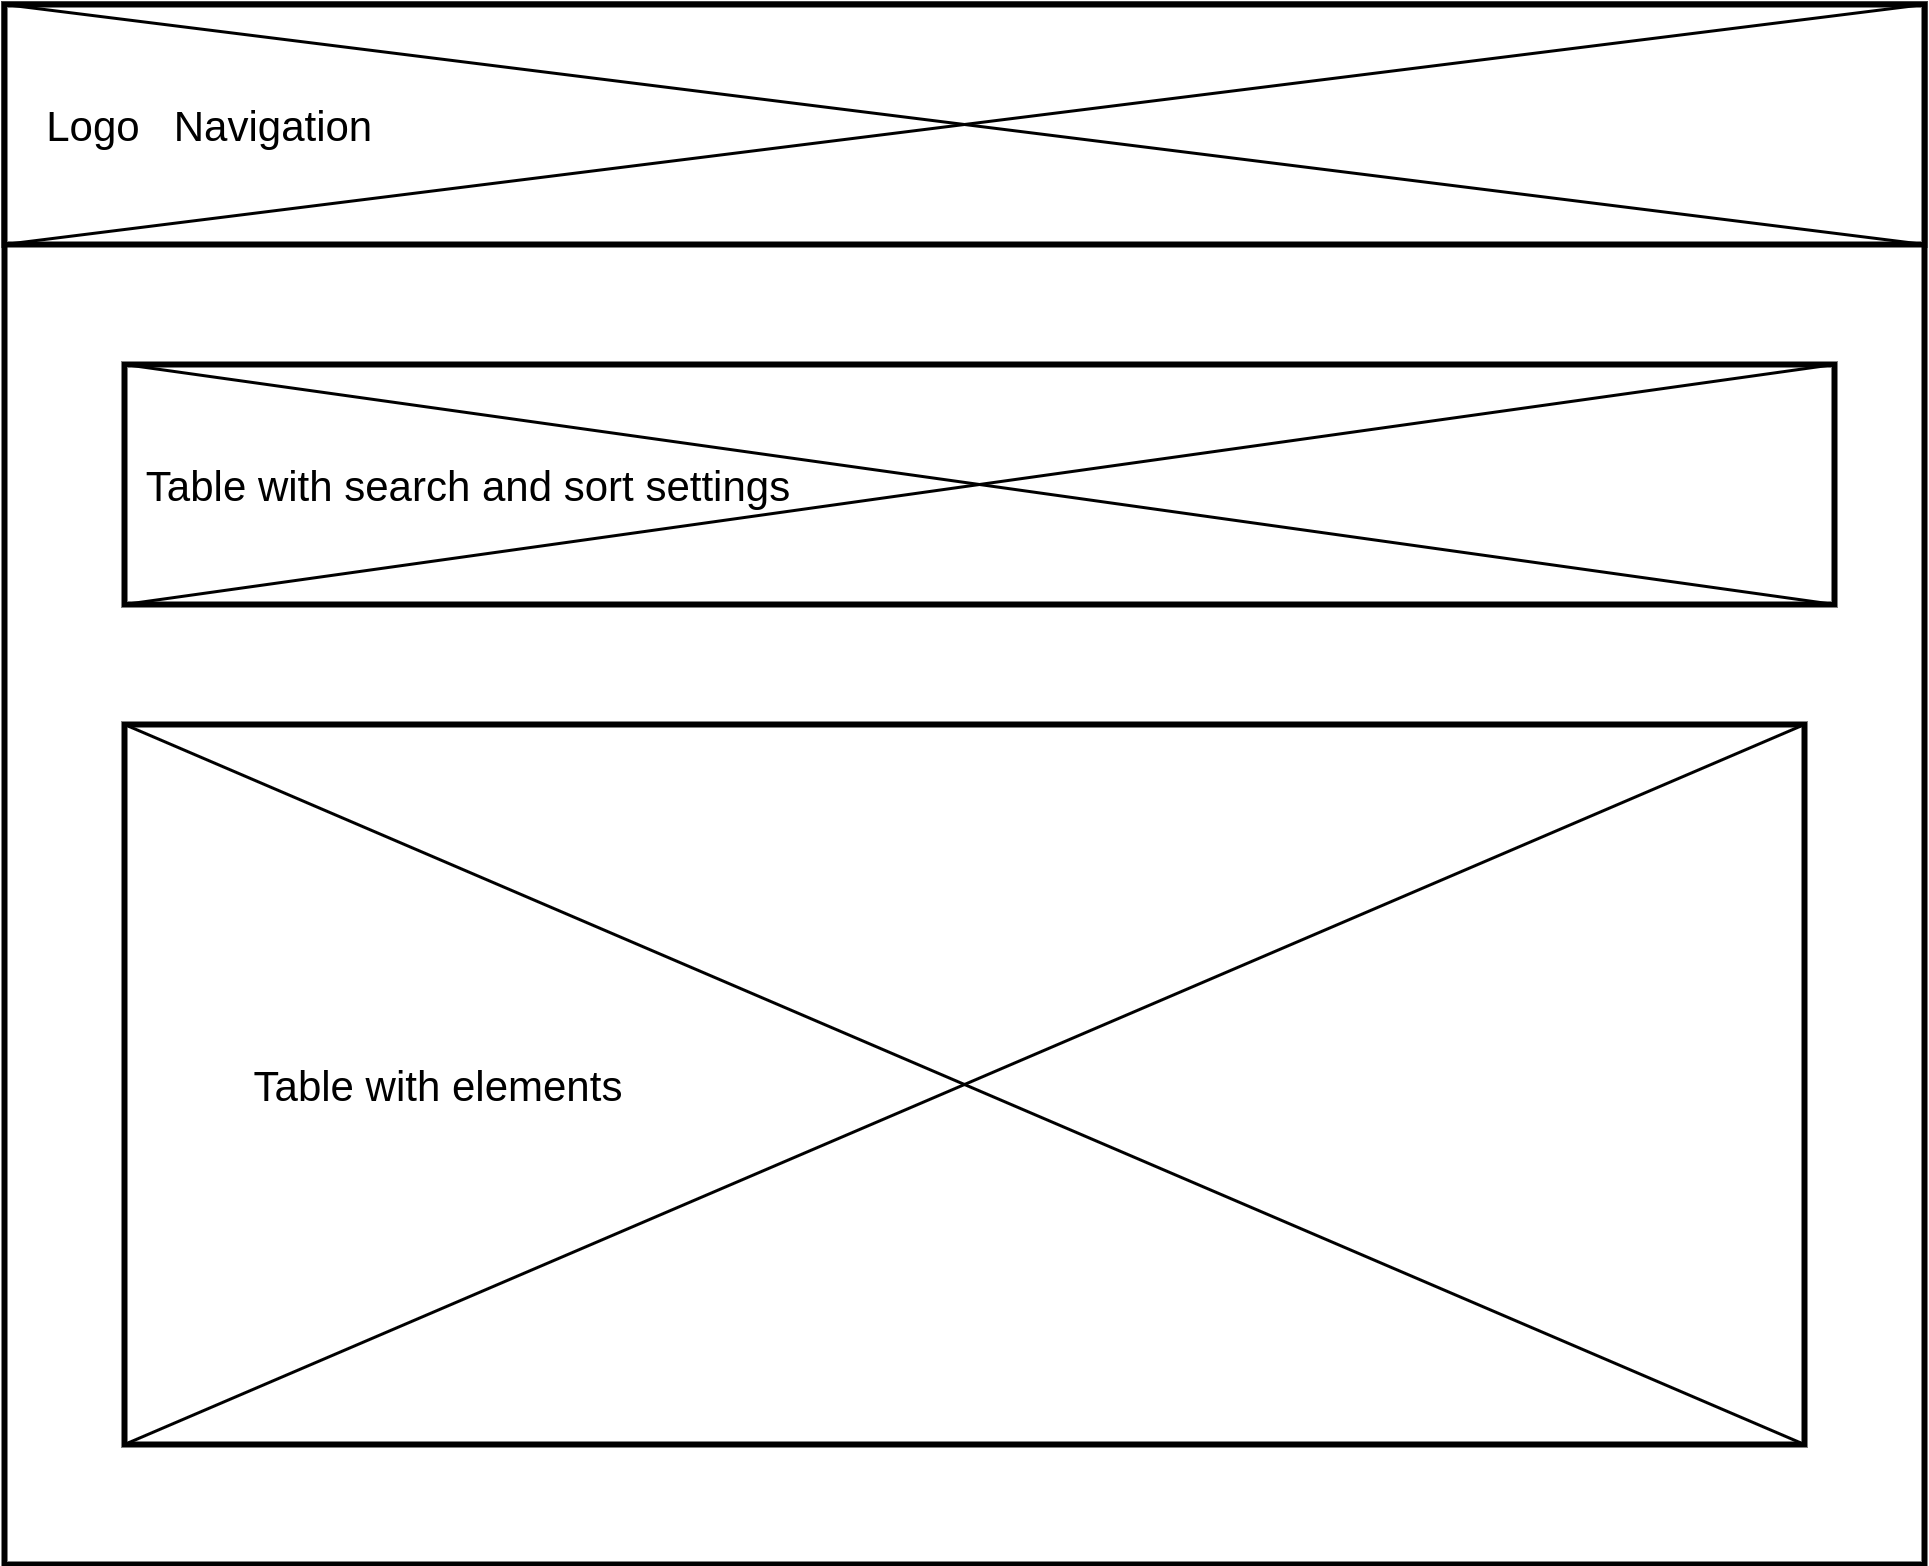
\includegraphics[width=15cm]
        {_input/formulationOfTheProblem/projectUI/layout.png}
    }
    \caption{Макет страницы}
    \label{fig:layoyt}
\end{figure}